\documentclass[a4paper]{article}
\usepackage[utf8]{inputenc}
\usepackage[a4paper,top=3cm,bottom=2cm,left=3cm,right=3cm,marginparwidth=1.75cm]{geometry}
\title{Neutron Simulations}
\author{Jack Sanders }
\date{Gas Lab 2021}
\usepackage{hyperref}
\usepackage{natbib}
\usepackage{mhchem}
\usepackage{graphicx}
\usepackage{subfig}
\usepackage{float}
\usepackage[toc,page]{appendix}

\begin{document}

\maketitle
\tableofcontents
\section{Introduction}
This document contains important plots from the studies carried out over summer 2021. This document will also contain the locations for all the files that are produced on the eprex server.

\section{Modifications to the simulation}
A few modifications were made to the simulation to fulfil the briefs of the study.
\subsection{macro file}
First the macro had to be setup to allow for neutrons to produced randomly across the surface of the sphere:
\begin{verbatim}
/gun/initialParticle neutron
/gun/initialEnergy 0.000025 keV
\end{verbatim}
The energy of the neutrons is also chosen, with the energy for thermal being shown above. To produce random initial conditions the following commands are used:
\begin{verbatim}
/gun/initialPositionSpherical 0 0 0 cm
/gun/initialDirectionSpherical 0 0 0
/gun/minRadius 16.01 cm
/gun/maxRadius 16.01 cm
\end{verbatim}
However this will produce particles in all directions, resulting in lost initial particles. This is corrected by calculating the dot product in PrimaryGeneratorAction shown in section \_\_.
The mac files used in all the studies can be found on the server at 
\begin{verbatim}
cd /disk/moose/newsg/sanders/localfiles/Software/
\end{verbatim}
\subsection{Run Action}
\begin{verbatim}
if(true) {
        std::ofstream outfile ("data.txt");
        outfile << "Volume, Process, Particle, Process, Radius, theta, phi, 
        SecondaryParent, EnergyDeposit" << std::endl;
        outfile << " \\\\\\\\\\\\\\\\\\\\  Run " << run->GetRunID() << " start. 
        ////////////////////" <<  std::endl;
        outfile.close();
};

\end{verbatim}
\subsection{Primary Generator Action}
Updates to this file are within the random direction function to remove nay directions that are pointing away from the sphere. The dot product checks if it is within $\pm$ 90 degrees.
\begin{verbatim}
if (m_randomDirection && !m_radialDir) {  // Randomised initial direction
//    double cosTheta0dir = G4RandFlat::shoot(-1.0, 1.0);
//    double phi0dir = G4RandFlat::shoot(0.0, 2. * acos(-1));
    double theta0pos = acos(m_initialPosition.cosTheta());
    double phi0pos = m_initialPosition.phi();
    double cosTheta0dir, phi0dir;
    while(true) {
        cosTheta0dir = G4RandFlat::shoot(-1.0, 1.0);
        phi0dir = G4RandFlat::shoot(0.0, 2. * acos(-1));

        double theta0dir = acos(cosTheta0dir);
        //double dot = sin(theta0dir)*sin(theta0pos)*cos(phi0dir-phi0pos)
        +cos(theta0dir)*cos(theta0pos);
        double dottheta = cos(theta0pos-theta0dir);
        double dotphi = cos(phi0pos-phi0dir);
        if( dottheta > 0 and dotphi > 0 ){
        //if( dot > 0 ){
                break;
        }else {
                continue;
    }
    }
\end{verbatim}
This can be found:
\begin{verbatim}
less /disk/moose/newsg/sanders/localfiles/Software/simulationg4
/SPC_Simulation/src/PrimaryGeneratorAction.cc
\end{verbatim}
\subsection{Event Action}
\begin{verbatim}
if(true) {
 std::ofstream outfile;
 outfile.open("data.txt", std::ios_base::app);
 //std::ofstream outfile("data");
 //outfile.open("test.txt", std::ios_base::app); // append instead of overwrite
 outfile << "================= EVENT " << evtNb + 1
            << " =================" << std::endl;
 outfile.close();
};

\end{verbatim}
\begin{verbatim}
less /disk/moose/newsg/neutron_simulation/localfiles/Software/simulationg4/
SPC_Simulation/src/EventAction.cc
\end{verbatim}
\subsection{Stepping Action}
\begin{verbatim}
if(true) {
 if( step->GetDeltaEnergy() != 0 && pv->GetName() != "World" && (ke-ke_post) > 0 && SP != 11) {
                std::ofstream outfile;
                outfile.open("data.txt", std::ios_base::app); // append instead of overwrite
                double SParticle = step->GetTrack()->GetDynamicParticle()->GetPDGcode();
                G4String PVolume = pv->GetName();
                G4String PProcess=  postPoint->GetProcessDefinedStep()->GetProcessName();
                //G4String SProcess = postPoint->GetProcessDefinedStep()->GetProcessName();
                G4ThreeVector newPos = G4ThreeVector(x1, z1, y1);
                double SParent = step->GetTrack()->GetParentID();
                double SRadius = (newPos.r() / cm);
                double theta = newPos.cosTheta();
                double phi = newPos.phi();
                //double ket = ke-ke_post;
                outfile << std::fixed;
                if( step->GetTrack()->GetParentID() == 0 ) {
                outfile << "Primary "<< ',' <<  PVolume  << ',' << PProcess << ',' << SParticle  
                << ',' << SRadius <<',' << theta << ',' << phi << ',' << SParent << ',' 
                << edep << std::endl;
                outfile.close();
                } else if (step->GetTrack()->GetParentID() != 0) {
                outfile << "Secondary "<< ','  <<  PVolume  << ',' << PProcess << ',' 
                << SParticle << ',' << SRadius <<',' << theta << ',' 
                << phi << ',' << SParent << ',' << edep << std::endl;
                outfile.close();

};
\end{verbatim}
\begin{verbatim}
less /disk/moose/newsg/sanders/localfiles/Software/simulationg4/
SPC_Simulation/src/SteppingAction.cc
\end{verbatim}
\section{Galactic vs Steel}
A study was carried out to identify what in the data is produced from the sphere. In the simulation it is possible to change the material of the cathode (sphere). Here we used both "G4\_Galactic" and "G\_4 Stainless\_Steel". For this investigation, a single 2mm anode is used,
\begin{figure}[H]
    \centering
    \begin{minipage}{.5\textwidth}
        \centering
        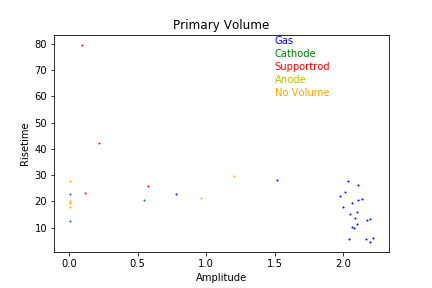
\includegraphics[width=1\linewidth]{GalacvSteel/galac.png}
        \caption{Amplitude vs Rise Time from run with galactic sphere}
        \label{fig:prob1_6_2}
    \end{minipage}%
    \begin{minipage}{0.5\textwidth}
        \centering
        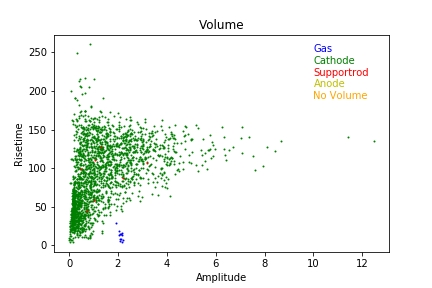
\includegraphics[width=1\linewidth]{GalacvSteel/steel.png}
        \caption{Amplitude vs Rise Time from run with steel sphere}
        \label{fig:prob1_6_1}
    \end{minipage}
\end{figure}
\noindent Here is a good example to see the effect of the steel sphere on the signal produced from the detector. The large green region is missing in the galactic sphere with only the interactions within the gas. Even though compared to the next sections this used a single anode rather than the achinos it is clear to see that this would have the same effect. 
\subsection{Slides:}
\url{https://docs.google.com/presentation/d/1TpeoVpAiW5vhaxY8A20iGuLHqI-9jz2eBD6iUEo7P-g/edit?usp=sharing}
\section{Thermal Neutron Study}
The thermal neutrons were produced using 0.000025 keV neutrons on the surface of the steel sphere. 500000 neutrons have been simulated to allow for reasonable statistics and have produced the following plots.
\begin{figure}[H]-
        \centering
        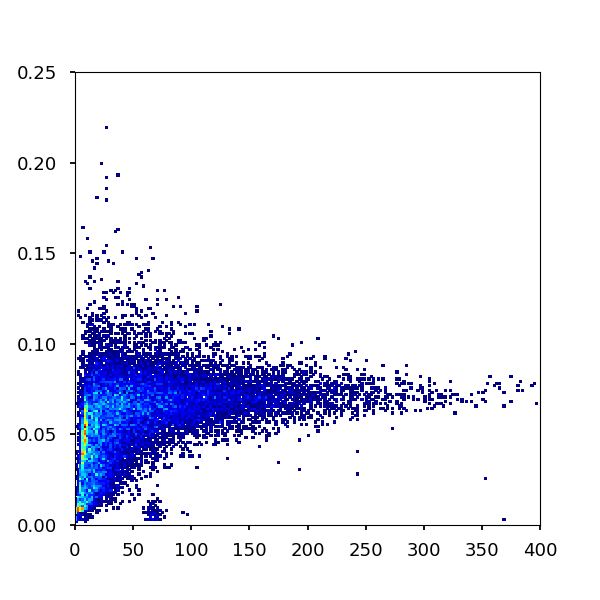
\includegraphics[height=10cm]{steel_achinos-2d.png}
        \caption{South Amplitude vs Rise time produced from simulation }
        \label{fig:south2d}
        \end{figure}
\begin{figure}[H]-
        \centering
        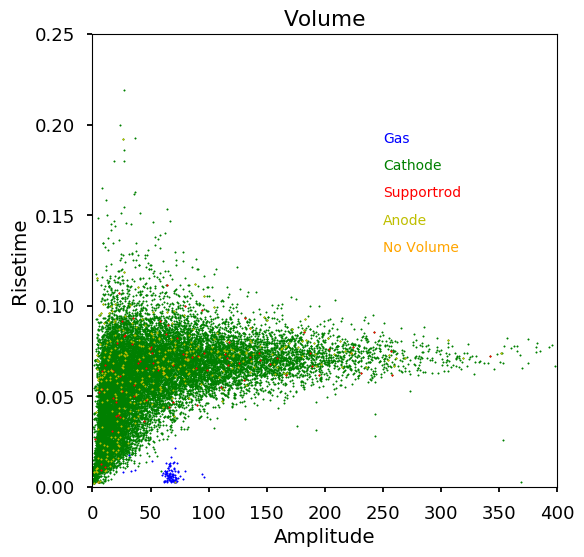
\includegraphics[height=10cm]{steel_achinos_vol_38.png}
        \caption{South Amplitude vs Rise time produced from simulation characterised with primary process}
        \label{fig:south2dpp}
        \end{figure}
Looking at the two plots above, the large population spread across the amplitude is produced from interactions of the neutron within the cathode. These interactions are usually scattering with some type of ionisation that produces electrons that pass into the gas and produce the signal. However this is slightly speculation as the code does not track electrons due to the large number produced within interactions and the avalanche region causing memory issues. 
\newline A clear distribution can be seen around 70 ADU which interacts within the gas volume. 
\begin{figure}[H]-
        \centering
        \includegraphics[height=10cm]{steel_achinos_gas_south.png}
        \caption{South Amplitude vs Rise time produced from simulation with only interactions from the gas}
        \label{fig:south2d}
        \end{figure}
\noindent This is important to use when comparing with the experimental data but is hard to analyse all the interacts as some are only across the North hemisphere (Far), producing a negative signal on the South (Near) sensor. Using the total amplitude that is calculated from both sensors, we can select specific interactions and investigate what has produced them.

\begin{figure}[H]-
        \centering
        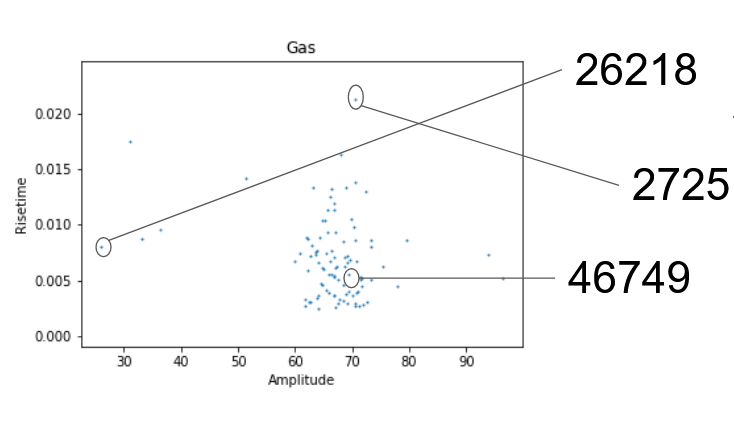
\includegraphics[height=10cm]{Capturegas.PNG}
        \caption{Total Amplitude vs Rise time produced from simulation with only interactions from the gas}
        \label{fig:south2d}
        \end{figure}
\subsection{Visualise}
\subsubsection{ID 26218}
This has an id of 26218 which is the position within the root file allowing to find the specific job and interaction.
\begin{figure}[H] 
  \label{ fig7} 
  \begin{minipage}[b]{0.5\linewidth}
    \centering
    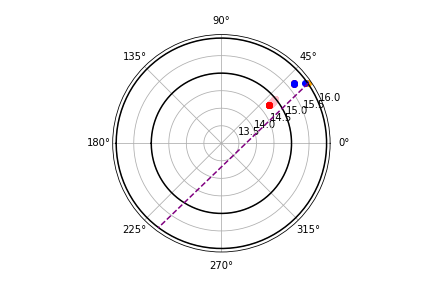
\includegraphics[width=1\linewidth]{id 26218/26_2_phi.png} 
    \caption{Plot of interactions in phi dimension} 
    \vspace{4ex}
  \end{minipage}%%
  \begin{minipage}[b]{0.5\linewidth}
    \centering
    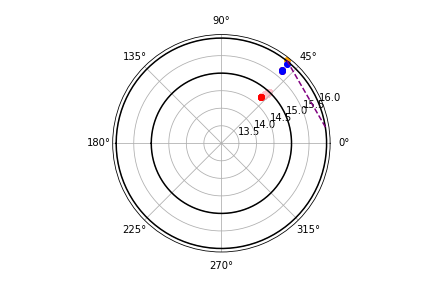
\includegraphics[width=1\linewidth]{id 26218/26_2_theta.png} 
    \caption{Plot of interactions in theta dimension} 
    \vspace{4ex}
  \end{minipage} 
  \begin{minipage}[b]{0.5\linewidth}
    \centering
    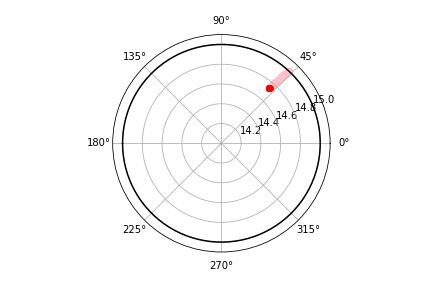
\includegraphics[width=1\linewidth]{id 26218/achinos_26218_phi.png} 
    \caption{Zoomed in plot of interactions in phi dimension} 
    \vspace{4ex}
  \end{minipage}%% 
  \begin{minipage}[b]{0.5\linewidth}
    \centering
    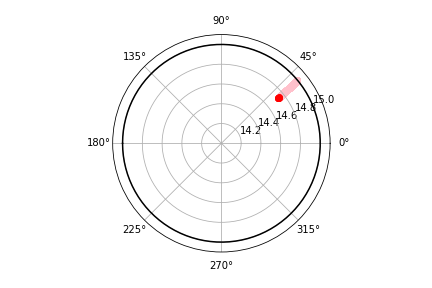
\includegraphics[width=1\linewidth]{id 26218/achinos_26218_theta.png} 
    \caption{Zoomed in plot of interactions in theta dimension} 
    \vspace{4ex}
  \end{minipage} 
\end{figure}
\noindent The plots above show the interactions within the spherical coordinates. Each point on the plot is an interaction a particle has with the detector, and each colour corresponds with a specific interaction:
\begin{itemize}
    \item[] Pink- hIoni
    \item[] Blue - hadElastic
    \item[] Yellow - NeutronInelastic
    \item[] Red - IonIoni
    \item[] Green - Photoelectric
\end{itemize}
\noindent This interaction is really interesting, the fact that it clearly shows the wall effect in action. Here the neutron inelastic scatters within the gas producing a proton that ionises the gas which is shown in pin. However the track/proton reaches the wall before all the energy is deposited within the detector which results in a much lower amplitude compared to the main distribution, such as id 46749.
\subsubsection{ID 46749}
\begin{figure}[H]
    \centering
    \begin{minipage}{.5\textwidth}
        \centering
        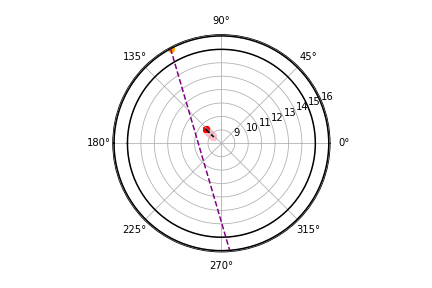
\includegraphics[width=1\linewidth]{id 46749/achinos_46749_phi.png}
        \caption{Plot of interactions in phi dimension}
        \label{fig:prob1_6_2}
    \end{minipage}%
    \begin{minipage}{0.5\textwidth}
        \centering
        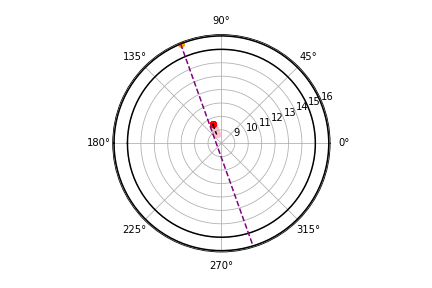
\includegraphics[width=1\linewidth]{id 46749/achinos_46749_theta.png}
        \caption{Plot of interactions in theta dimension}
        \label{fig:prob1_6_1}
    \end{minipage}
\end{figure}
\noindent Here this interaction producing a signal that fall within the denser region of points. The track describes this as its a ordinary track within the gas with all the energy of the proton being deposited within the gas. However the direction of the tracks also can effect the signal which is shown in id 2725
\begin{figure}[H]-
        \centering
        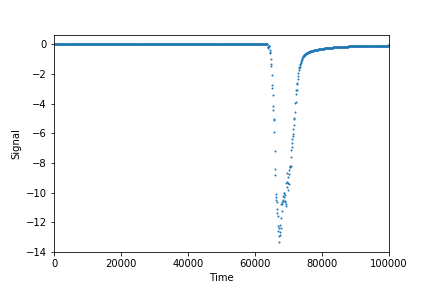
\includegraphics[height=5cm]{id 46749/signal_2045.png}
        \caption{Signal produced from the above interaction}
        \label{fig:south2dpp}
        \end{figure}
\subsubsection{ID 2725}
\begin{figure}[H]
    \centering
    \begin{minipage}{.5\textwidth}
        \centering
        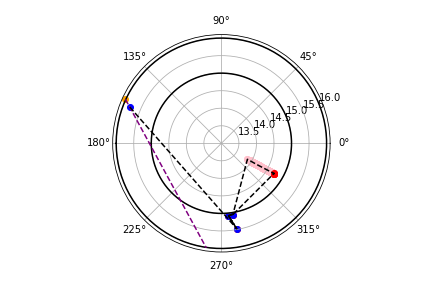
\includegraphics[width=1\linewidth]{id 2725/achinos_2725_phi.png}
        \caption{Plot of interactions in phi dimension}
        \label{fig:prob1_6_2}
    \end{minipage}%
    \begin{minipage}{0.5\textwidth}
        \centering
        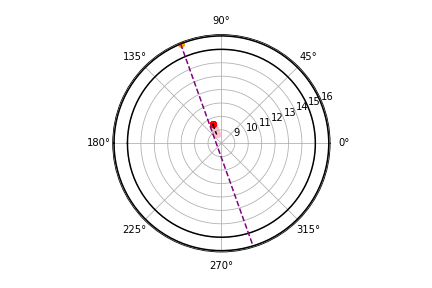
\includegraphics[width=1\linewidth]{id 46749/achinos_46749_theta.png}
        \caption{Plot of interactions in theta dimension}
        \label{fig:prob1_6_1}
    \end{minipage}
\end{figure}
\noindent Here the amplitude is similar to the majority of interactions but the rise time is much greater, which is expected when looking at the track as it is directed towards the centre meaning ion pairs are at different radius along the track. 
\subsection{Comparison with experimental}
The reasoning for this study is to compare the experimental data produced using the same initial conditions. The experimental data is from a run at 1\,Bar at 3800V which produced amplitude vs rise time plots below,
\begin{figure}[H]-
        \centering
        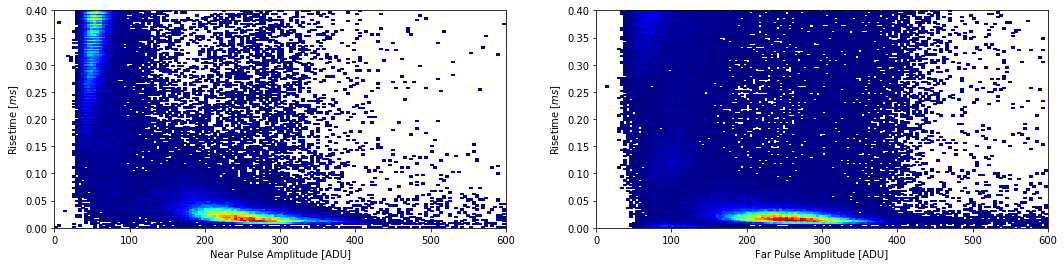
\includegraphics[width=1\linewidth]{uk24n001_risehigh.png}
        \caption{Experimental data from 3800V run}
        \label{fig:south2d}
        \end{figure}
\noindent Comparing the plots produced experimentally with the simulation, neither the amplitudes nor the rise time matches. Certain other parameters could be changes with diffusion within the avalanche being investigated in later section. The amplitude looks like there's a scaling factor that is different which become more obvious within the alpha study in a later section where as with the rise time this looks like the simulation doesn't completely match with the experimental data.
\newline However the simulation does show similar regions such as with the lower rise time neutron region appearing in both the simulation and experimental, with a higher rise time region atop it, which the simulation suggests is produced by the neutron scattering within the wall of the sphere. 
\begin{figure}[H]-
        \centering
        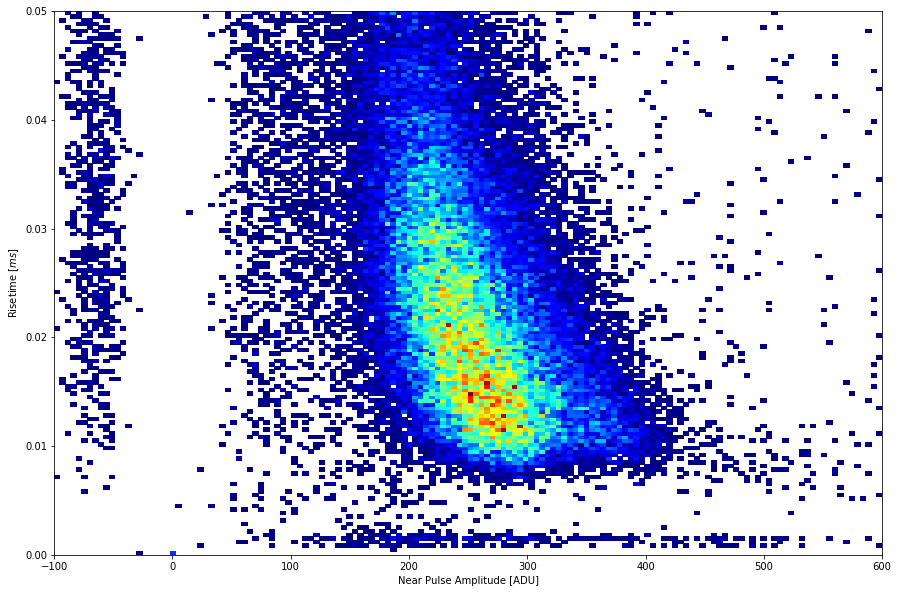
\includegraphics[height=10cm]{uk24n001_rt_wout_phantom_2.png}
        \caption{Experimental data from 3800V run zoomed in on the neutron peak}
        \label{fig:south2d}
        \end{figure}
\subsection{Summary}
\begin{itemize}
    \item {} 
\end{itemize}
\subsection{Links}
Slides: 
\begin{itemize}
    \item[] \url{https://docs.google.com/presentation/d/1yubwVUnTS2mEz1m5dvpc5Ar-2fx7prAqJKjLMpRyH_k/edit?usp=sharing}
\end{itemize}
\section{Diffusion Comparison}
Due to the disparity of rise time between the experimental and simulated data, it was thought that this could be caused by not including the diffusion with the avalanche region. The thinking is that diffusion would increase the rise time and also spread out each region to match the experimental data.
\begin{figure}[H]-
        \centering
        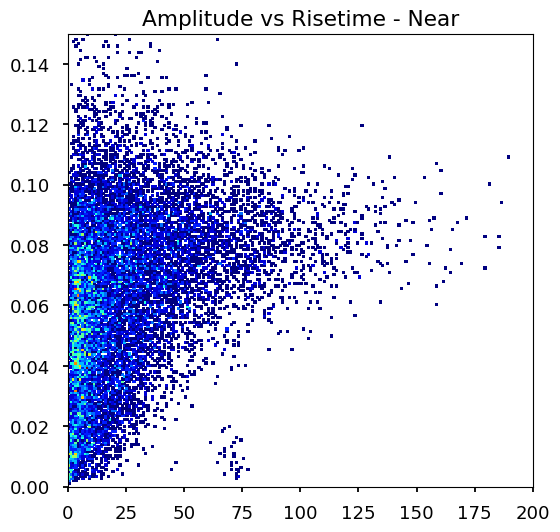
\includegraphics[width=1\linewidth]{diff/steel_achinos-2d_South_diff.png}
        \caption{Amplitude vs Rise time with diffusion within the avalanche region}
        \label{fig:south2d}
        \end{figure}
\noindent However when comparing the plots produced with diffusion on and without, there is not much difference between the rise time of each regions. Other reasons would have to be investigated into what caused this difference.
\newline On the slides found in the link below the north sensor is also compared, this was not included as it is believe that the north sensor of the experimental data has much greater noise compared to that of the south. 
\subsection{Links}
Slides: \url{https://docs.google.com/presentation/d/1nbNzZ2IsEBuv3AYV1iVgk0RYVXxPIv5x4xW5c3aR59c/edit?usp=sharing}
\section{Radon Measurements}
As known, the filter introduces Radon 222 into the detector volume with the nitrogen gas. The decay of radon produces alphas at a number of energies 
\begin{figure}[H]-
        \centering
        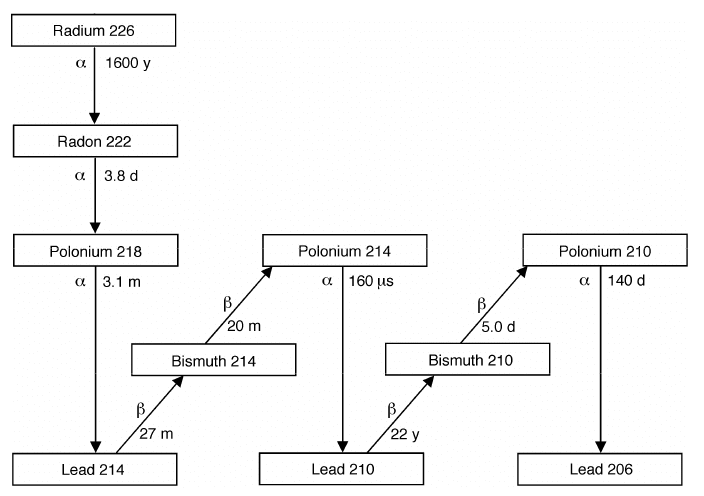
\includegraphics[width=1\linewidth]{Radon/radon.png}
        \caption{Radon Decay Scheme}
        \label{fig:south2d}
        \end{figure}
\noindent The first alpha decay from 222 produces and alpha of 5489.48 keV. Second from the decay of Polonium 218 at 6002.35 keV and finally from the Polonium 214 at 7686.82 keV. Due to the the long half life of the lead 210 this is as far as we need to investigate, unless for very long experiments.
\begin{figure}[H]-
        \centering
        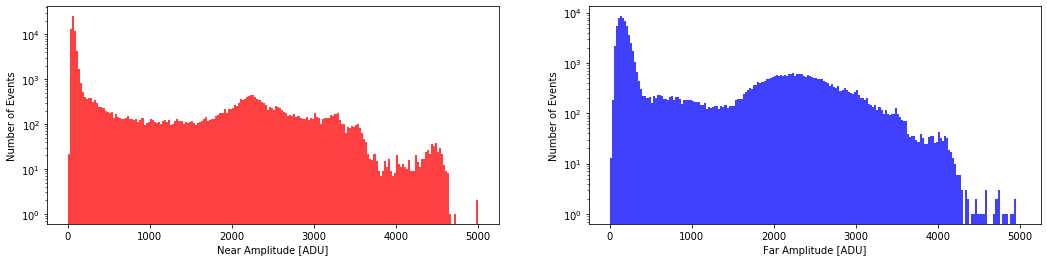
\includegraphics[width=1\linewidth]{Radon/va28n002_ampbefore.png}
        \caption{Amplitude histogram from background run a day after detector being filled - va28n002}
        \label{fig:south2d}
        \end{figure}
\begin{figure}[H]-
        \centering
        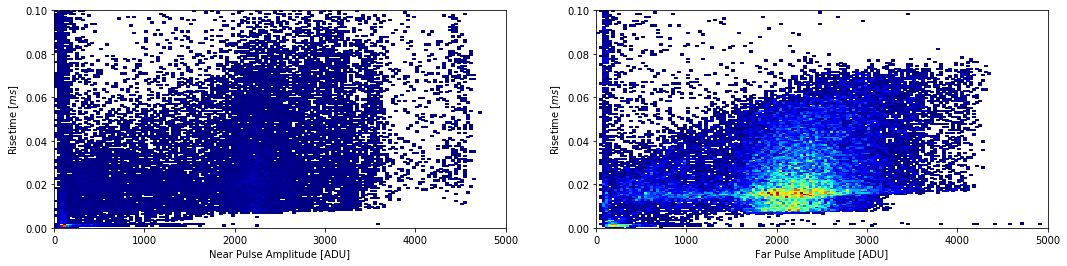
\includegraphics[width=1\linewidth]{Radon/va28n002_rise_.png}
        \caption{Amplitude vs Rise produced from background run}
        \label{fig:south2d}
        \end{figure}
\noindent In the rise time plots you can see there are a few distinct regions and can be slightly seen in the amplitude histogram. Using the expected alpha energies, you can predict where these would fall compared to the others. First the large region around 2250 ADU was selected as the lower energy alpha, 
\begin{figure}[H]-
        \centering
        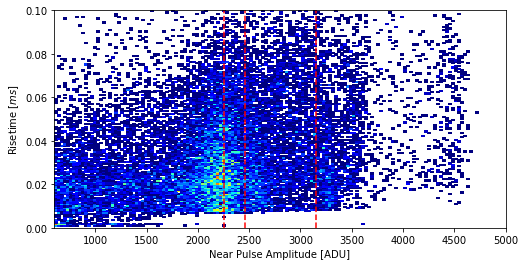
\includegraphics[width=1\linewidth]{Radon/va28n002_rise_lineslow.png}
        \caption{Near channel Amplitude vs Rise time plots with estimated alpha energies}
        \label{fig:south2d}
        \end{figure}
\noindent Here the lines don't really fall on the regions, with the distinct region being much higher amplitude that could be achieved if this dense region was the lower alpha energy. So the far region is selected as the higher alpha energy,
\begin{figure}[H]-
        \centering
        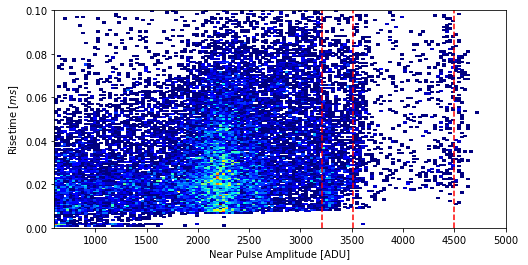
\includegraphics[width=1\linewidth]{Radon/va28n002_rise_lineshigh.png}
        \caption{Near channel Amplitude vs Rise time plots with estimated alpha energies}
        \label{fig:south2d}
        \end{figure}
\noindent Here the lines do fall mostly on the distinct regions at the higher amplitudes. Here the middle line falls on a distinct line and the lower energy falling of its expected line slightly. This suggests that the lower dense region is produced from some other process other than the decay of the radon within the gas. 
\newline So to simulate this we select the lower energy alphas and the higher energy alphas. To simulate this, a few important notes would have to be taken into account. As the radon 222 is distributed throughout the gas we can initiate the simulation by randomising the starting position anywhere in the gas and directed all around. To do this the dot product function that was produced was turned off to allow direction 2 pi all around. The higher energy alpha is much different, it is not really distributed throughout the gas due to the multiple decays and is mainly found around the edge of the gas volume. For simulation, the alphas were then produced on the edge of the gas at 14.99 cm away from the centre still with the dot product turned off. 
\begin{figure}[H]
    \centering
    \begin{minipage}{.5\textwidth}
        \centering
        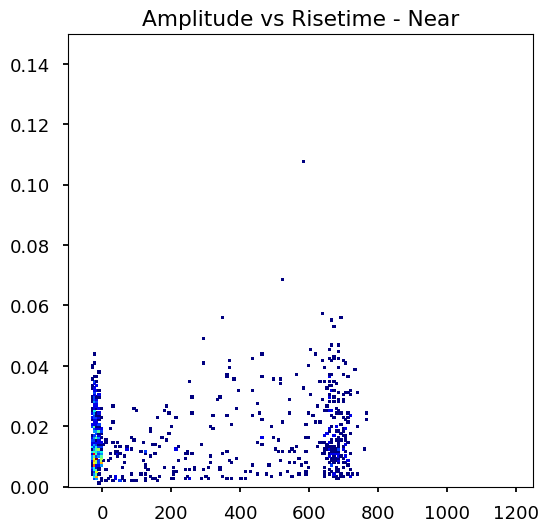
\includegraphics[width=1\linewidth]{Radon/steel_achinos-2d_South_alpha3.png}
        \caption{Near channel Amplitude vs Rise Time of 5489 keV alpha}
        \label{fig:prob1_6_2}
    \end{minipage}%
    \begin{minipage}{0.5\textwidth}
        \centering
        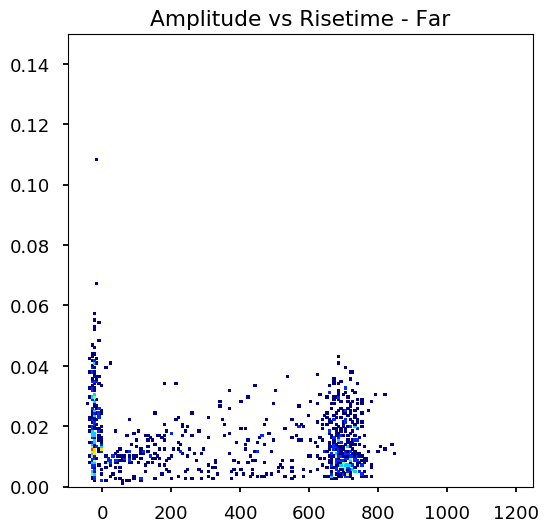
\includegraphics[width=1\linewidth]{Radon/steel_achinos-2d_North_alpha3.png}
        \caption{Far channel Amplitude vs Rise Time of 5489 keV alpha}
        \label{fig:prob1_6_1}
    \end{minipage}
\end{figure}
\noindent Comparing these alpha energies, the amplitude of the lower alpha is around 680 ADU. Using ratios of the alpha energies the higher alpha energy can be predicted to be 952 ADU. This is very close to what was produced in the figure below with the region being around 960 ADU.
\begin{figure}[H]
    \centering
    \begin{minipage}{.5\textwidth}
        \centering
        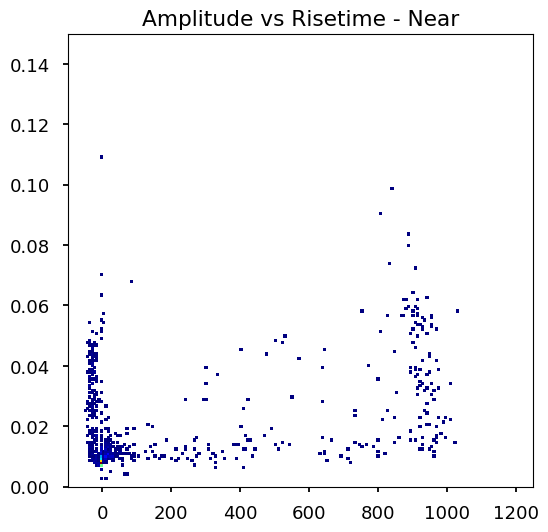
\includegraphics[width=1\linewidth]{Radon/steel_achinos-2d_South_alpha2.png}
        \caption{Near channel Amplitude vs Rise Time of 7686  keV alpha}
        \label{fig:prob1_6_2}
    \end{minipage}%
    \begin{minipage}{0.5\textwidth}
        \centering
        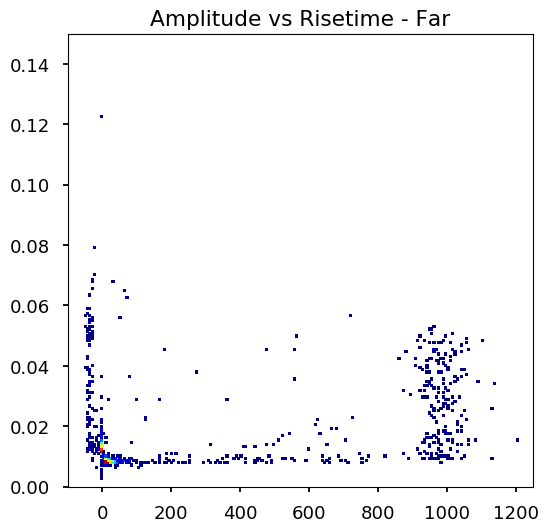
\includegraphics[width=1\linewidth]{Radon/steel_achinos-2d_North_alpha2.png}
        \caption{Far channel Amplitude vs Rise Time of 7686  keV alpha}
        \label{fig:prob1_6_1}
    \end{minipage}
\end{figure}
\noindent Obviously it is hard to compare this to the experimental data as the intensity of each band is different due to the decay of the radon. To get a full view of whats happening during the decay of the radon, a full simulation of the decay within the gas volume would have to be carried out.
\newline However now a comparison can be made between the thermal neutrons and the radon to investigate if the amplitude discrepancy can be fixed by just scaling the amplitude. First a comparison of the experimental data was done,
\begin{figure}[H]
    \centering
    \begin{minipage}{.5\textwidth}
        \centering
        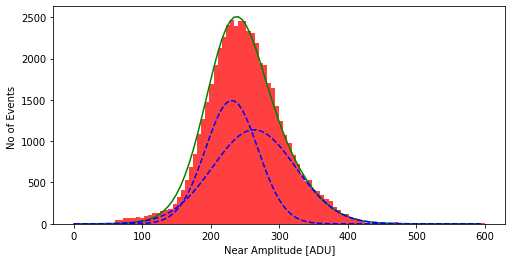
\includegraphics[width=1\linewidth]{Radon/uk24n001_amp2.png}
        \caption{Near channel Amplitude vs Rise Time of thermal neutron run at 3800V}
        \label{fig:prob1_6_2}
    \end{minipage}%
    \begin{minipage}{0.5\textwidth}
        \centering
        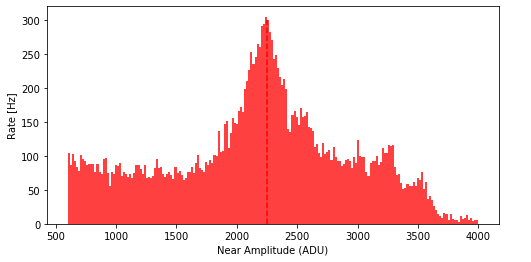
\includegraphics[width=1\linewidth]{Radon/va28n002_alphas2.png}
        \caption{Near channel Amplitude vs Rise Time of just background at 3800V}
        \label{fig:prob1_6_1}
    \end{minipage}
\end{figure}
\noindent The thermal neutron amplitude peak is at around 250 ADU and the neutron is around 2250 ADU. Resulting in the thermal neutron peak being around 0.11 times smaller than the alpha peak. This can then be compared to the simulation, 
\begin{figure}[H]
    \centering
    \begin{minipage}{.5\textwidth}
        \centering
        \includegraphics[width=1\linewidth]{Radon/steel_achinos_gas_south.png}
        \caption{Near channel Amplitude vs Rise Time of interactions occurring in the gas}
        \label{fig:prob1_6_2}
    \end{minipage}%
    \begin{minipage}{0.5\textwidth}
        \centering
        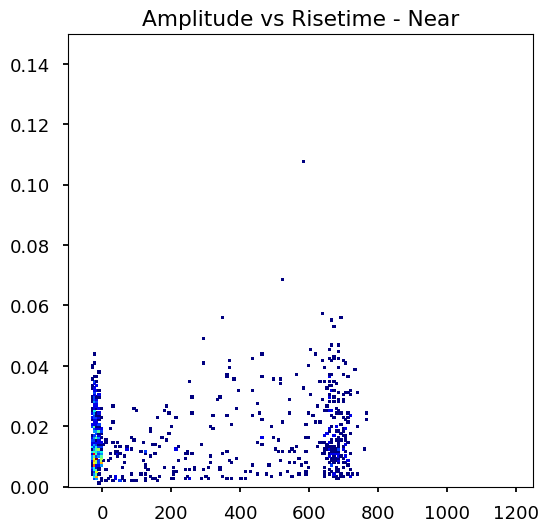
\includegraphics[width=1\linewidth]{Radon/steel_achinos-2d_South_alpha3.png}
        \caption{Near channel Amplitude vs Rise Time of 5489 keV alpha}
        \label{fig:prob1_6_1}
    \end{minipage}
\end{figure}
\noindent In the simulation the thermal neutron peak is around 70 ADU, compared to the alpha peak at 680 ADU. Producing a ratio of around 0.10, which is very comparable to that of the experimental data, suggesting that the amplitude can be fixed just with a scaling factor.
\subsection{Links}
Slides: \url{https://docs.google.com/presentation/d/1FE1MNsuQWdtsKqmDutoXnv7PLjWUE3w3C-c1u3eMviY/edit?usp=sharing}
\section{Fast Neutron Study}
The neutron source used is americium241-beryllium9 (Am-Be). Chosen for the Am alpha decay and the Be low Z, which interacts with the alpha producing a neutron \cite{nrc},
\begin{equation}
    \ce{^{9}B} + \alpha \rightarrow \ce{^{12}C} + n + 4.44MeV \gamma
\end{equation}
Which has the characteristics,
\begin{itemize}
    \item[] {Half-life: $432.2\,y$}
    \item[] {Source activity: $1\,Curie = 3.7 \times 10^{10}\,Bq$}
    \item[] {Average neutron energy: $4.2\,MeV$}
\end{itemize}
The material is held within a X3 stainless steel capsule shown in Figure \ref{fig:ambe}, with dimensions $d = 22.4\,mm$ and $h = 31\,mm$. The case decreases the neutron output for the source to $2.6 \times 10^{6}\,Bq$ but keeps the source contained. Due to the high average neutron energy it is important that the source be kept in a radiation box when not being used due to the high average energy of the neutron.
\begin{figure}[H]-
    \centering
    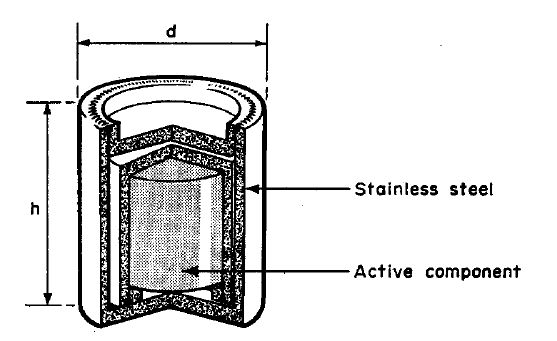
\includegraphics[height=5cm]{Fast/ambe.PNG}
    \caption{Diagram of Am-Be source contained within a stainless steel capsule}
    \label{fig:ambe}
\end{figure}
\noindent This is taken from my dissertation and has references there.
\newline The neutron energy spectrum of the Am-Be source is shown below,
\begin{figure}[H]-
        \centering
        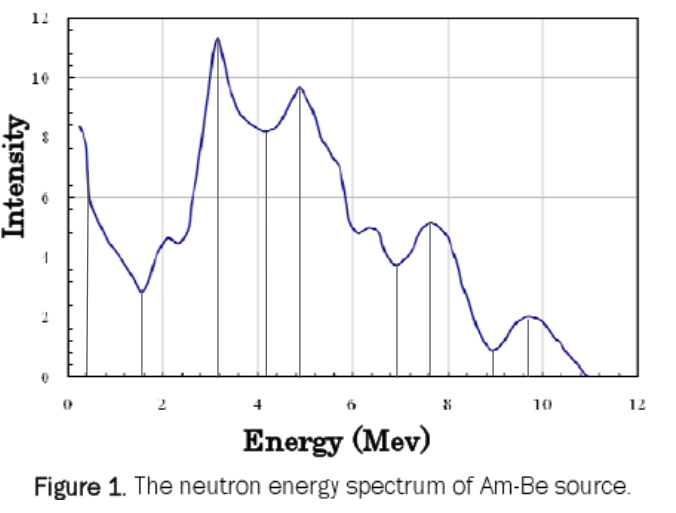
\includegraphics[width=1\linewidth]{Fast/spectrum.PNG}
        \caption{Plot of Am-Be neutron energy spectrum}
        \label{fig:south2d}
        \end{figure}
\noindent The spectrum has a number of features that are selected to be simulated, chosen from the  peaks and troughs of the spectrum. The energies selected are:
\begin{itemize}
    \item 0.4 MeV
    \item 3.2 MeV
    \item 4.2 MeV
    \item 4.9 MeV
    \item 6.9 MeV
    \item 7.6 MeV
    \item 9 MeV
    \item 9.7 MeV
\end{itemize}
\noindent At first the energies were simulated with an initial 100,000 neutrons with the exception of the first two which have more which will be explained later on. 
\subsection{0.4 MeV}
\begin{figure}[H]
    \centering
    \begin{minipage}{.5\textwidth}
        \centering
        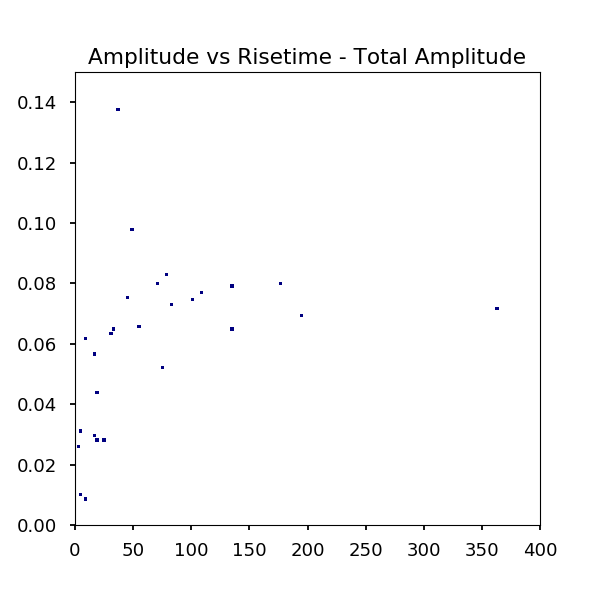
\includegraphics[width=1\linewidth]{Fast/steel_achinos-2d_fast.png}
        \caption{Amplitude vs rise time 2d hist for 0.4 MeV neutrons}
        \label{fig:prob1_6_2}
    \end{minipage}%
    \begin{minipage}{0.5\textwidth}
        \centering
        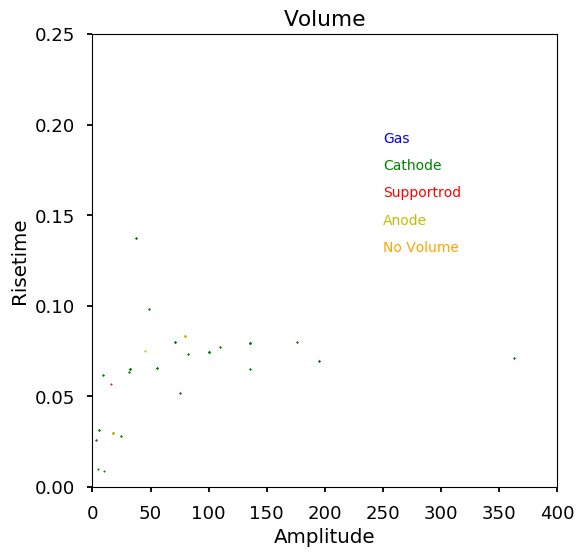
\includegraphics[width=1\linewidth]{Fast/steel_achinos_vol_38_fast.png}
        \caption{Amplitude vs rise time primary volume for 0.4 MeV neutrons}
        \label{fig:prob1_6_1}
    \end{minipage}
\end{figure}
\noindent At this energy there is not much interactions with the detector, with the any interactions being in the cathode, which as we know from previous plots is the most likely interaction within the detector. This low number of interactions can be explained by looking at the cross section of the nitrogen gas, 
\begin{figure}[H]-
        \centering
        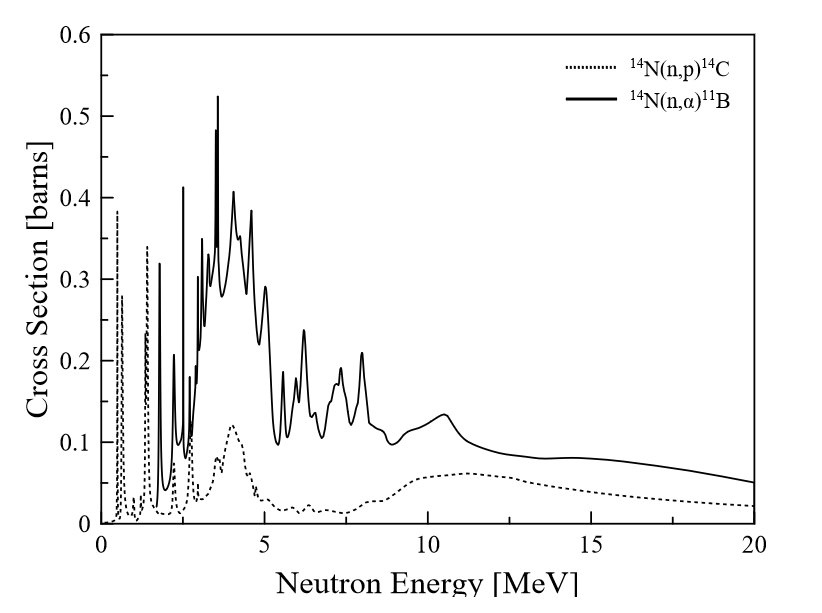
\includegraphics[width=1\linewidth]{Fast/cross.png}
        \caption{Cross section of neutrons with nitrogen gas}
        \label{fig:south2d}
        \end{figure}
\noindent The 0.4 MeV neutrons obviously fall within one of the low points on this plot resulting in the low number of interactions.
\subsection{3.2 MeV}
\begin{figure}[H]
    \centering
    \begin{minipage}{.5\textwidth}
        \centering
        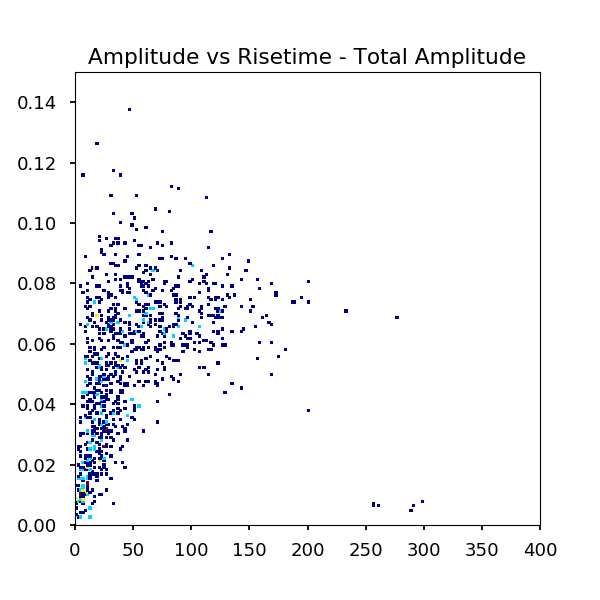
\includegraphics[width=1\linewidth]{Fast/steel_achinos-2d_fast-2.png}
        \caption{Amplitude vs rise time 2d hist for 3.2 MeV neutrons}
        \label{fig:prob1_6_2}
    \end{minipage}%
    \begin{minipage}{0.5\textwidth}
        \centering
        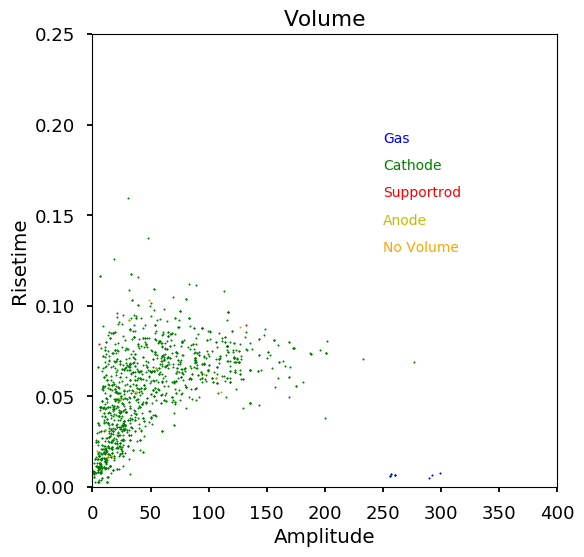
\includegraphics[width=1\linewidth]{Fast/steel_achinos_vol_38_fast-2.png}
        \caption{Amplitude vs rise time primary volume for 3.2 MeV neutrons}
        \label{fig:prob1_6_1}
    \end{minipage}
\end{figure}
\noindent The plots above are from 200,000 incident 3.2 MeV neutrons. This energy has had more incident neutrons as it is the highest probable neutron energy, so is important when understanding how the spectrum interacts within the detector. In the plots above, similar regions are seen such as the cathode interactions, that were also seen in the thermal neutrons simulation, but with the gas interactions producing much higher amplitudes. 
\begin{figure}[H]-
        \centering
        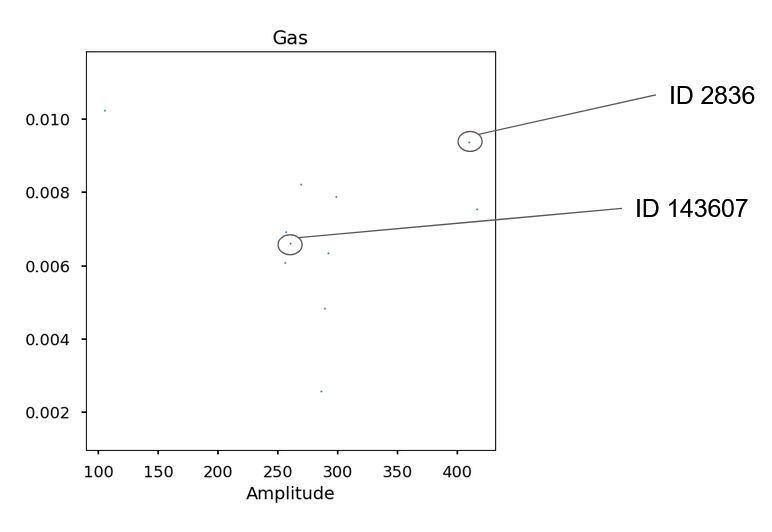
\includegraphics[width=1\linewidth]{Fast/gas-id-2.PNG}
        \caption{Amplitude vs rise time of gas interactions for 3.2 MeV neutrons}
        \label{fig:south2d}
        \end{figure}
\noindent Using the secondary data the interactions have been tracked, allowig for the differentation between different interactions that occur within the gas.
\subsubsection{Visualise ID 2836}
This is interaction produces an alpha as it is over the minimum energy for this interaction, 1.7 MeV. 
\begin{equation}
    \ce{^{14}N} + n \rightarrow \ce{^{11}B} + \alpha - 158keV
\end{equation}
\noindent Due to this interaction being endothermic the ionisation tracks are quite short, which are shown in plots below,
\begin{figure}[H]
    \centering
    \begin{minipage}{.5\textwidth}
        \centering
        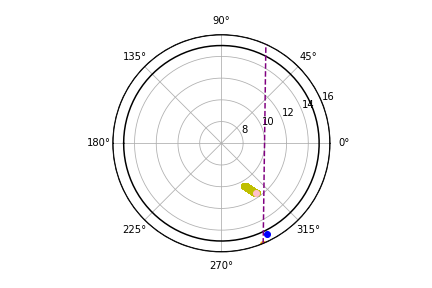
\includegraphics[width=1\linewidth]{Fast/2836_phi.png}
        \caption{Polar plot in the Phi dimension}
        \label{fig:prob1_6_2}
    \end{minipage}%
    \begin{minipage}{0.5\textwidth}
        \centering
        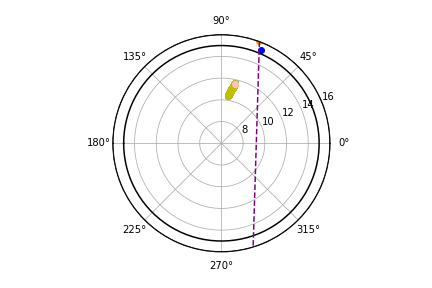
\includegraphics[width=1\linewidth]{Fast/2836_theta.png}
        \caption{Polar plot in the theta dimension}
        \label{fig:prob1_6_1}
    \end{minipage}
\end{figure}
\noindent The purple dotted line is the direction from the initial point on the surface of the sphere that the neutron travels. I believe that the reason for the direction not lining up with the interaction i the gas is due to scattering that is not being recorded, resulting in the neutron changing directions before the interaction occurs. It would be useful to know what is causing this but this would increase the file size exponentially. 
\subsubsection{Visualise ID 143607}
\begin{figure}[H]
    \centering
    \begin{minipage}{.5\textwidth}
        \centering
        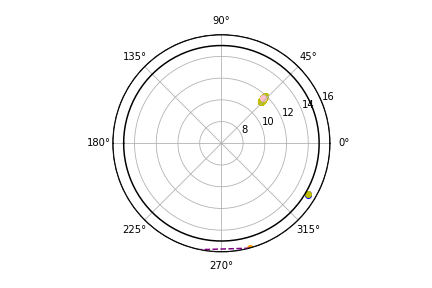
\includegraphics[width=1\linewidth]{Fast/143607_phi.png}
        \caption{Polar plot in the Phi dimension}
        \label{fig:prob1_6_2}
    \end{minipage}%
    \begin{minipage}{0.5\textwidth}
        \centering
        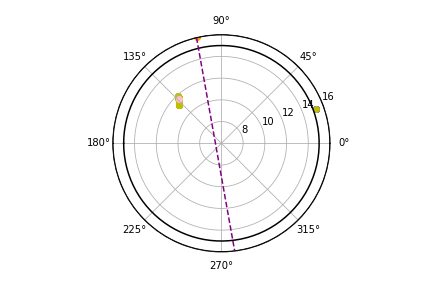
\includegraphics[width=1\linewidth]{Fast/143607_theta.png}
        \caption{Polar plot in the theta dimension}
        \label{fig:prob1_6_1}
    \end{minipage}
\end{figure}
\noindent Here the same interaction is occurring, but the neutron loses some energy from scattering within the cathode, resulting in a lower amplitude compared to the previous interaction.
\subsection{4.2 MeV}
\begin{figure}[H]
    \centering
    \begin{minipage}{.5\textwidth}
        \centering
        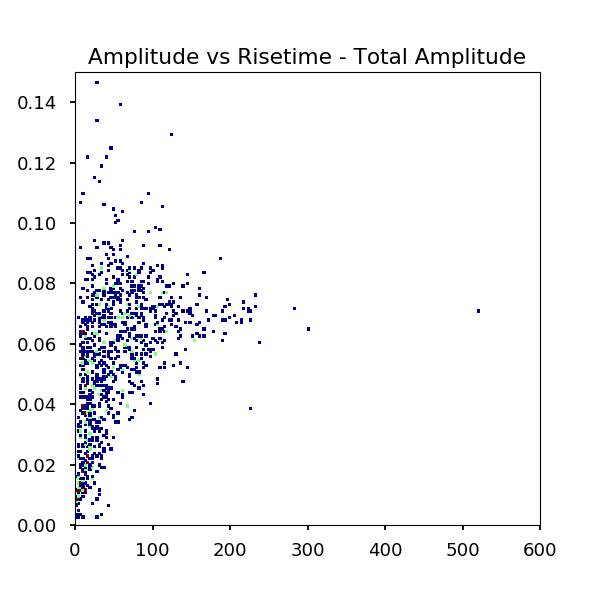
\includegraphics[width=1\linewidth]{Fast/steel_achinos-2d_fast-3.png}
        \caption{Amplitude vs rise time 2d hist for 4.2 MeV neutrons}
        \label{fig:prob1_6_2}
    \end{minipage}%
    \begin{minipage}{0.5\textwidth}
        \centering
        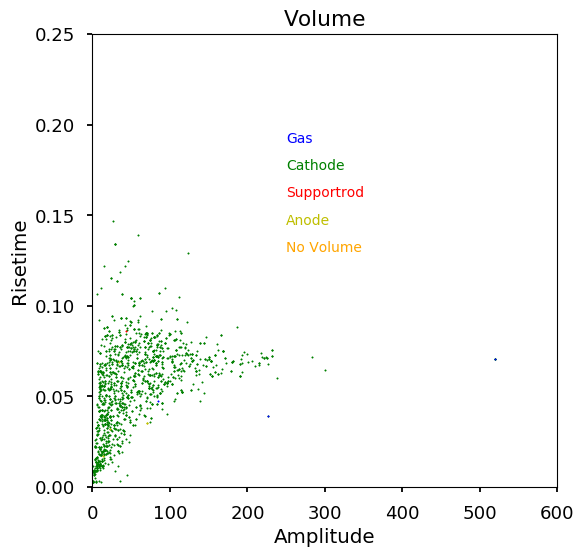
\includegraphics[width=1\linewidth]{Fast/steel_achinos_vol_38_fast-3.png}
        \caption{Amplitude vs rise time primary volume for 4.2 MeV neutrons}
        \label{fig:prob1_6_1}
    \end{minipage}
\end{figure}
\noindent Using the primary volume plot, the lower risetime gas interactions are not present as the interactions within the gas are at a much higher risetime, comparable the the interactions within the cathode. 
\begin{figure}[H]-
        \centering
        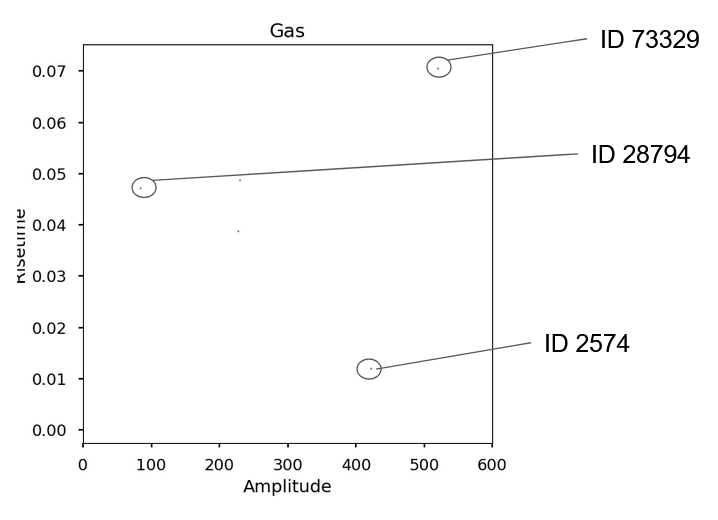
\includegraphics[width=1\linewidth]{Fast/gas-id-3.PNG}
        \caption{Amplitude vs rise time of gas interactions for 3.2 MeV neutrons}
        \label{fig:south2d}
        \end{figure}
\noindent the interactions in the gas have a large spread of rise times, with one at the expected rise time for the neutrons and a couple a higher rise times and can be explained when looking at the visualisations.  
\subsubsection{Visualise ID 2574}
\begin{figure}[H]
    \centering
    \begin{minipage}{.5\textwidth}
        \centering
        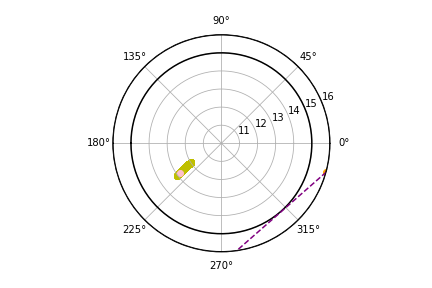
\includegraphics[width=1\linewidth]{Fast/2574_phi.png}
        \caption{Polar plot in the Phi dimension}
        \label{fig:prob1_6_2}
    \end{minipage}%
    \begin{minipage}{0.5\textwidth}
        \centering
        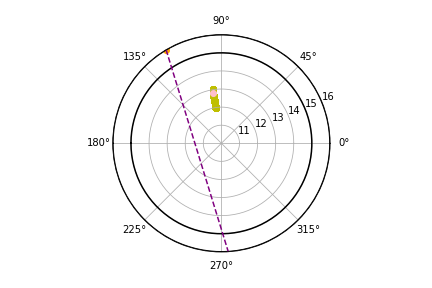
\includegraphics[width=1\linewidth]{Fast/2574_theta.png}
        \caption{Polar plot in the theta dimension}
        \label{fig:prob1_6_1}
    \end{minipage}
\end{figure}
\noindent Here this interaction is at the rise time expected for the neutrons seen in the previous energy and this is no exception. This interaction produces an alpha and doesn't seen to scatter to much in the cathode, suggesting most of the energy has been deposited into the detector.
\subsection{Visualise ID 28794}
\begin{figure}[H]
    \centering
    \begin{minipage}{.5\textwidth}
        \centering
        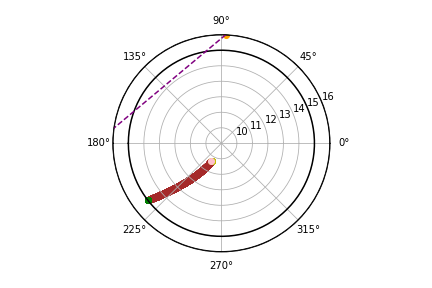
\includegraphics[width=1\linewidth]{Fast/28794_phi.png}
        \caption{Polar plot in the Phi dimension}
        \label{fig:prob1_6_2}
    \end{minipage}%
    \begin{minipage}{0.5\textwidth}
        \centering
        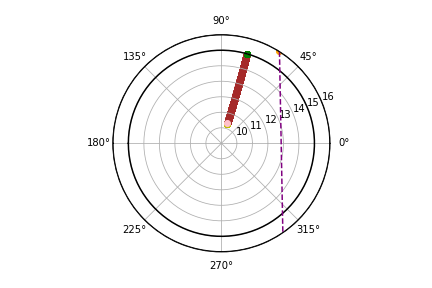
\includegraphics[width=1\linewidth]{Fast/28794_theta.png}
        \caption{Polar plot in the theta dimension}
        \label{fig:prob1_6_1}
    \end{minipage}
\end{figure}
\noindent This interaction is very interesting. This is interaction produced a proton through the same interaction used by thermal neutrons:
\begin{equation}
    \ce{^{14}N} + n \rightarrow \ce{^{14}C} + p + 625.87keV
    \label{eq:neu}
\end{equation}
\noindent Due to the exothermic reaction, the proton has a large amount of energy, allowing it to produce a long ionisation track. This also increases the chance of the proton hitting the wall before depositing all of its energy, which is what happened here. This is why the interaction has produced a point at lower energy due to the wall effect and the higher rise time, due to the long ionisation track.
\subsubsection{Visualise ID 73329}
\begin{figure}[H]
    \centering
    \begin{minipage}{.5\textwidth}
        \centering
        \includegraphics[width=1\linewidth]{Fast/73329_phi.png}
        \caption{Polar plot in the Phi dimension}
        \label{fig:prob1_6_2}
    \end{minipage}%
    \begin{minipage}{0.5\textwidth}
        \centering
        \includegraphics[width=1\linewidth]{Fast/73329_theta.png}
        \caption{Polar plot in the theta dimension}
        \label{fig:prob1_6_1}
    \end{minipage}
\end{figure}
\noindent This is another example of the proton interaction, suggesting that this energy is in a peak in the N(n,p)C cross section. This plot is a bit strange in that is seems to be repelled by the achinos in the centre, This interaction has a very long ionisation track producing the higher rise time, but it did deposit all the energy within the detector before the wall, which is why the amplitude is around that of the alpha interaction.
\subsection{4.9 MeV}
\begin{figure}[H]
    \centering
    \begin{minipage}{.5\textwidth}
        \centering
        \includegraphics[width=1\linewidth]{Fast/steel_achinos-2d_fast-4.png}
        \caption{Amplitude vs rise time 2d hist for 4.9 MeV neutrons}
        \label{fig:prob1_6_2}
    \end{minipage}%
    \begin{minipage}{0.5\textwidth}
        \centering
        \includegraphics[width=1\linewidth]{Fast/steel_achinos_vol_38_fast-4.png}
        \caption{Amplitude vs rise time primary volume for 4.9 MeV neutrons}
        \label{fig:prob1_6_1}
    \end{minipage}
\end{figure}
\noindent At this energy the interactions within the gas are much less spread out in terms of rise time, with no gas interactions at high rise time. Suggesting that the interactions don't include the proton interaction.
\begin{figure}[H]-
        \centering
        \includegraphics[width=.5\linewidth]{Fast/steel_achinos_gas3_fast-4.png}
        \caption{Amplitude vs rise time of gas interactions for 4.9 MeV neutrons}
        \label{fig:south2d}
        \end{figure}
\noindent A couple interactions have been investigated and can be found on the slides.
\subsection{6.9 MeV}
\begin{figure}[H]
    \centering
    \begin{minipage}{.5\textwidth}
        \centering
        \includegraphics[width=1\linewidth]{Fast/steel_achinos-2d_fast-7.png}
        \caption{Amplitude vs rise time 2d hist for 6.9 MeV neutrons}
        \label{fig:prob1_6_2}
    \end{minipage}%
    \begin{minipage}{0.5\textwidth}
        \centering
        \includegraphics[width=1\linewidth]{Fast/steel_achinos_vol_38_fast-7.png}
        \caption{Amplitude vs rise time primary volume for 6.9 MeV neutrons}
        \label{fig:prob1_6_1}
    \end{minipage}
\begin{figure}[H]-
        \centering
        \includegraphics[width=1\linewidth]{Fast/gas-id-7.PNG}
        \caption{Amplitude vs rise time of gas interactions for 6.9 MeV neutrons}
        \label{fig:south2d}
        \end{figure}
\end{figure}
\noindent The ID numbers 4721 and 10868 are both interactions that produce alphas with ID 95912 being different completely. The alpha interactions can be found on the slide below.
\subsubsection{Visualise ID 95912}
\begin{figure}[H]
    \centering
    \begin{minipage}{.5\textwidth}
        \centering
        \includegraphics[width=1\linewidth]{Fast/95912_phi.png}
        \caption{Polar plot in the Phi dimension}
        \label{fig:prob1_6_2}
    \end{minipage}%
    \begin{minipage}{0.5\textwidth}
        \centering
        \includegraphics[width=1\linewidth]{Fast/95912_theta.png}
        \caption{Polar plot in the theta dimension}
        \label{fig:prob1_6_1}
    \end{minipage}
\end{figure}
\noindent Here the neutron is in-elastically scattering with the nitrogen gas but instead of interaction though the processes mentioned before, the nitrogen atom recoils and this atom is what causes the ionisation track. This results in a very small track and in turn a smaller rise time.
\subsection{7.6 Mev}
\begin{figure}[H]
    \centering
    \begin{minipage}{.5\textwidth}
        \centering
        \includegraphics[width=1\linewidth]{Fast/steel_achinos-2d_fast-8.png}
        \caption{Amplitude vs rise time 2d hist for 7.6 MeV neutrons}
        \label{fig:prob1_6_2}
    \end{minipage}%
    \begin{minipage}{0.5\textwidth}
        \centering
        \includegraphics[width=1\linewidth]{Fast/steel_achinos_vol_38_fast-8.png}
        \caption{Amplitude vs rise time primary volume for 7.6 MeV neutrons}
        \label{fig:prob1_6_1}
    \end{minipage}
\end{figure}
\noindent This energy is similar to the energy before with interactions producing an alpha and also recoils of the nitrogen atoms. The visualisation of the interactions can be found on the slides from the link below.
\begin{figure}[H]-
        \centering
        \includegraphics[width=1\linewidth]{Fast/gas-id-8.PNG}
        \caption{Amplitude vs rise time of gas interactions for 7.6 MeV neutrons}
        \label{fig:south2d}
        \end{figure}
\subsection{9 MeV}
\begin{figure}[H]
    \centering
    \begin{minipage}{.5\textwidth}
        \centering
        \includegraphics[width=1\linewidth]{Fast/steel_achinos-2d_fast-8.png}
        \caption{Amplitude vs rise time 2d hist for 9 MeV neutrons}
        \label{fig:prob1_6_2}
    \end{minipage}%
    \begin{minipage}{0.5\textwidth}
        \centering
        \includegraphics[width=1\linewidth]{Fast/steel_achinos_vol_38_fast-8.png}
        \caption{Amplitude vs rise time primary volume for 9 MeV neutrons}
        \label{fig:prob1_6_1}
    \end{minipage}
\end{figure}
\noindent There is only two interactions within the gas, probably due to the cross section at this energy, with the interaction ID 64671 being produced by the recoil of a nitrogen atom which can be seen on the slides.
\begin{figure}[H]-
        \centering
        \includegraphics[width=1\linewidth]{Fast/gas-id-5.PNG}
        \caption{Amplitude vs rise time of gas interactions for 9 MeV neutrons}
        \label{fig:south2d}
        \end{figure}
\subsubsection{Visualise ID 2284}
\begin{figure}[H]
    \centering
    \begin{minipage}{.5\textwidth}
        \centering
        \includegraphics[width=1\linewidth]{Fast/2284_phi.png}
        \caption{Polar plot in the Phi dimension}
        \label{fig:prob1_6_2}
    \end{minipage}%
    \begin{minipage}{0.5\textwidth}
        \centering
        \includegraphics[width=1\linewidth]{Fast/2284_theta.png}
        \caption{Polar plot in the theta dimension}
        \label{fig:prob1_6_1}
    \end{minipage}
\end{figure}

\noindent Here is another example of the interaction that produces a proton which is then producing the ionisation track. Due to the long track produced by the high energy proton it again reaches the wall before depositing all its energy within the volume, producing a lower amplitude on the amplitude vs rise tie plot. However again we see this curve round the detector which suggests that the proton is being effected by the electric field produced from the achinos event though it has been said that this doesn't occur in the simulation. To check this isn't just a illusion form the projection of the plot a Cartesian plot was made,
\begin{figure}[H]-
        \centering
        \includegraphics[width=1\linewidth]{Fast/Cart_3D.png}
        \caption{3D Cartesian of the interaction with ID 2284}
        \label{fig:south2d}
        \end{figure}
\noindent This shows that the protons track is curved and looks very similar to that of a particle within a electric field.
\subsection{9.7 MeV}
\begin{figure}[H]
    \centering
    \begin{minipage}{.5\textwidth}
        \centering
        \includegraphics[width=1\linewidth]{Fast/steel_achinos-2d_fast-6.png}
        \caption{Amplitude vs rise time 2d hist for 7.6 MeV neutrons}
        \label{fig:prob1_6_2}
    \end{minipage}%
    \begin{minipage}{0.5\textwidth}
        \centering
        \includegraphics[width=1\linewidth]{Fast/steel_achinos_vol_38_fast-6.png}
        \caption{Amplitude vs rise time primary volume for 7.6 MeV neutrons}
        \label{fig:prob1_6_1}
    \end{minipage}
\end{figure}
\begin{figure}[H]-
        \centering
        \includegraphics[width=1\linewidth]{Fast/gas-id-6.PNG}
        \caption{Amplitude vs rise time of gas interactions for 9.7 MeV neutrons}
        \label{fig:south2d}
        \end{figure}
\subsection{Future Work}
At the moment there is data for each separate energy, however it has to be scaled to the intensities produced from the Am-Be source. In order to keep some statistics with this it is vital that the highest intensity has a reasonably high number of incident neutrons to allow for the low intensity energy's to have some statistics. I have made a plan on what incident neutrons are needed to then combine to represent what is produced fro the source:
\begin{figure}[H]-
        \centering
        \includegraphics[width=1\linewidth]{Fast/init.PNG}
        \caption{Plans for initial neutrons}
        \label{fig:south2d}
        \end{figure}
\noindent It would also be good to select energies from the cross section, especially where there is a peak in order to fill in any gaps.
\subsection{Links}
Slides: \url{https://docs.google.com/presentation/d/1gW2tr8RMD1AOCVlkp-i58RAN4fYuXECy5f9TJ0Emblw/edit?usp=sharing}
\begin{appendices}
\section{How to visualise}
First task is to find the id of the event, which is done in the python file when the events are separated for the primary volume. When you have an id you can then find the specific job using the log found here and the first number of the id, 
\begin{verbatim}
less /disk/moose/newsg/neutron_fastneutrons/log1-20.txt
\end{verbatim}
\noindent Then the rest of the Numbers can be identified using the log found here, 
\begin{verbatim}
less /disk/moose/newsg/neutron_fastneutrons/sublog.txt
\end{verbatim}
\noindent This allows for the selection of the data file found in the job directory which contains all the secondary data. The visualise python file take both the job root file and the specific data file and will produce plots that describes the tracks.
\newline Most of the time the numbers match up but especially for the fast neutrons there are a few missing events due to problems of the server so if the file cant be found a linux search can be used in the specific job,
\begin{verbatim}
grep -r 'Gas' data_*
\end{verbatim}
\end{appendices}
\bibliographystyle{IEEEtran}
\bibliography{references} 
\end{document}
